\documentclass[final]{beamer}

% ====================
% Packages
% ====================

\usepackage[T1]{fontenc}
\usepackage{lmodern}
\usepackage[french=quotes]{csquotes} \MakeOuterQuote{"}
\usepackage[orientation=portrait,size=a0,scale=1.0]{beamerposter}
\usetheme{gemini}
\usecolortheme{nott}
\usepackage{graphicx}
\usepackage{booktabs}
\usepackage{tikz}
\usepackage{multicol}
\usepackage{pgfplots}
\usepackage[inkscapeformat=png]{svg}
\pgfplotsset{compat=1.14}
\usepackage{anyfontsize}
\usepackage{xcolor}
\usepackage[skip=2pt,font=normalsize]{subcaption}
\usepackage{adjustbox}
\usepackage{tabularx}
\usepackage{caption}
\usepackage{tabularx}
\usepackage{changepage}
\usepackage[english]{babel}
\captionsetup{font=it}

\usepackage{makecell}
\renewcommand\theadalign{bc}
\renewcommand\theadfont{\bfseries}
\renewcommand\theadgape{\Gape[4pt]}
\renewcommand\cellgape{\Gape[4pt]}

%%%

\usepackage{listings}
\usepackage{xcolor}

\definecolor{codegreen}{rgb}{0,0.6,0}
\definecolor{codegray}{rgb}{0.5,0.5,0.5}
\definecolor{codepurple}{rgb}{0.58,0,0.82}
\definecolor{backcolour}{rgb}{0.95,0.95,0.92}

\lstdefinestyle{mystyle}{
    backgroundcolor=\color{backcolour},
    commentstyle=\color{codegreen},
    keywordstyle=\color{magenta},
    numberstyle=\tiny\color{codegray},
    stringstyle=\color{codepurple},
    basicstyle=\footnotesize,
    breakatwhitespace=false,
    breaklines=true,
    captionpos=b,
    keepspaces=true,
    numbers=left,
    numbersep=5pt,
    showspaces=false,
    showstringspaces=false,
    showtabs=false,
    tabsize=2
}

\lstset{style=mystyle}


%%%

% \setbeamersize{text margin left=30mm,text margin right=30mm} 

% \addtobeamertemplate{block begin}{%
%   \setlength{\textwidth}{1.2\textwidth}%
%   \leftskip=10pt\rightskip=10pt\vspace{10pt}
%   \par\vspace{10pt}
% }{}


% \setbeamertemplate{itemize/enumerate body begin}{\normalsize}
% \setbeamertemplate{itemize/enumerate subbody begin}{\normalsize}
% \setbeamertemplate{itemize/enumerate subsubbody begin}{\normalsize}

\usepackage{tikz}
\usetikzlibrary{shapes.geometric, arrows}

% Defining Tickz Style
\tikzstyle{startstop} = [rectangle, rounded corners, minimum width=3cm, minimum height=1cm, text centered, text width=10cm, draw=white, fill=white]

% \tikzstyle{io} = [trapezium, trapezium left angle=70, trapezium right angle=110, minimum width=3cm, minimum height=1cm, text centered, text width=4.5cm, draw=black, fill=blue!30 ]

\tikzstyle{process} = [rectangle, minimum width=3cm, minimum height=1cm, text centered, text width=6cm, draw=black, fill=white, text width=10cm]

% \tikzstyle{decision} = [diamond, minimum width=3cm, minimum height=1cm, text centered, draw=black, fill=green!30]

\tikzstyle{arrow} = [ultra thick,->,>=stealth]


% ====================
% Lengths
% ====================

% If you have N columns, choose \sepwidth and \colwidth such that
% (N+1)*\sepwidth + N*\colwidth = \paperwidth
\newlength{\sepwidth}
\newlength{\colwidth}
\setlength{\sepwidth}{-2ex}
\setlength{\colwidth}{0.45\paperwidth}

\newcommand{\separatorcolumn}{\begin{column}{\sepwidth}\end{column}}


\newenvironment{variableblock}[3]{%
    \setbeamercolor{block body}{#2}
    \setbeamercolor{block title}{#3}
    \begin{block}{#1}}{\end{block}}

\addtobeamertemplate{block begin}
{
    \setlength{\textwidth}{1.07\textwidth}%
}
{%\vspace{1ex plus 0.5ex minus 0.5ex} % Pads top of block
    % separates paragraphs in a block
    %\setlength{\parskip}{24pt plus 1pt minus 1pt}%
    \begin{adjustwidth}{0.5cm}{0.5cm}
        }
        \addtobeamertemplate{block end}
        {\end{adjustwidth}%
    \vspace{1ex plus 0.5ex minus 0.5ex}
}% Pads bottom of block
{}
%{\vspace{10ex plus 1ex minus 1ex}} % Seperates blocks from each other

% ====================
%Title
% ====================

\title{De l'Organisation d'un Système Multi-Agent de Cyberdéfense}

\author{\textbf{Julien Soulé} \inst{1,2} \and Jean-Paul Jamont \inst{1} \and Michel Occello \inst{1} Paul Théron \inst{3} Louis-Marie Traonouez \inst{2}}

\institute[shortinst]{\inst{1} Univ. Grenoble Alpe, Grenoble INP, LCIS, Valence, France \samelineand \inst{2} Thales Land and Air Systems, BL IAS, Rennes, France \samelineand \inst{3} AICA IWG, La Guillermie, France}


% ====================
% Footer (optional)
% ====================

\footercontent{
    % \href{https://www.lipsum.com}{\textbf{https://www.lipsum.com}} \hfill

    % \raggedgauche

    % \textbf{Conclave de doctorat Connect 2023} \hfill

    \textbf{\underline{Contact :}} \ \href{mailto:julien.soule@lcis.grenoble-inp.fr}{\textit{julien.soule@lcis.grenoble-inp.fr}}}
% (peut être laissé de côté pour supprimer le pied de page)

\logoright{
\includegraphics[height=3cm]{logos/grenoble-inp_logo.png}}
{
\includegraphics[height=2cm]{logos/lcis_logo.png}}
{
\includegraphics[height=3.5cm]{logos/uga_logo.jpg}}
{
\includegraphics[height=3.5cm]{logos/la-ruche_logo.png}}

\begin{document}

\begin{frame}[t]

\vspace{-2ex}

\begin{columns}[t]
    \separatorcolumn

\hspace{-1ex}

\begin{column}{\colwidth}

    \begin{variableblock}{Contexte}{bg=lightgray,fg=black}{bg=lightgray,fg=black}

        \begin{itemize}

            \item \headingNoLine{Systèmes avec une surface d'attaque importante}
                  \begin{itemize}
                      \item Objets connectés (IoT/IoBT), drones, domotique, véhicules tout-terrain, etc.
                      \item Infrastructures cybernétiques, hétérogènes et distribuées
                  \end{itemize}

            \item \headingNoLine{Réagir aux cyberattaques en cours : cyberdéfense}
                  \begin{itemize}
                      \item Charges de travail importantes à traiter en peu de temps, etc.
                      \item Interruption de communication, brouillage, etc.
                  \end{itemize}

                  \quad $\Longrightarrow$ Besoin de : \headingNoLine{réactivité, flexibilité, autonomie, choix de stratégies...}

                  \

            \item \headingNoLine{Système Multi-Agents de Cyberdéfense (SMAC)} :

                  \begin{itemize}

                      \item Agents dotés de compétences/connaissances différentes mais atteignant un objectif commun grâce à la coopération, l'interaction et l'organisation

                      \item Fournir des moyens de gérer l'ouverture, l'évolutivité et l'autonomie du système hôte en déléguant différents aspects de la cyberdéfense aux agents

                  \end{itemize}

                  \

                  \begin{figure}
                      \centering
                      % \includegraphics[width=0.9\columnwidth]{images/MASCARA_Organization.pdf}
                      \includesvg[width=0.8\columnwidth]{images/MAS_definition_illustration.svg}
                      \caption{Vue schématique d'un système multi-agent de cyberdéfense en action}
                      \label{fig:mon_étiquette}
                  \end{figure}

                  % \vspace{-1ex}

            \item \headingNoLine{Agent de cyberdéfense intelligent autonome} (AICA)

                  \begin{itemize}
                      \item "\textbf{AICA IWG}" (cf \url{https://www.aica-iwg.org/}) ayant succédé au \textit{Groupe de travail de recherche IST-152} de l'OTAN qui se concentrait sur les "Agents intelligents, autonomes et de confiance pour la cyberdéfense et la résilience".
                  \end{itemize}

                  % \vspace{-2ex}

        \end{itemize}

        % \begin{figure}
        % \centering
        % % \includegraphics[width=0.9\columnwidth]{images/MASCARA_Organization.pdf}
        % \includesvg[width=\columnwidth]{images/MASCARA Organisation.svg}
        % \caption{Architecture de référence AICA}
        % \label{fig:mon_étiquette}
        % \end{figure}

    \end{variableblock}

    \begin{variableblock}{Revue SMA de cyberdéfense}{bg=lightorange,fg=black}{bg=lightorange,fg=black}

        \begin{itemize}

            % \item \textbf{Objectif} : Analyse des MAS de cyberdéfense disponibles pour trouver les relations entre l'organisation, les objectifs de cyberdéfense et l'environnement de déploiement.

            \item \textbf{Dans plus de 60\% des ouvrages connexes :}
                  \begin{itemize}
                      \item Objectifs de cyberdéfense se concentrent sur \textbf{détection des anomalies et intrusions}
                      \item \textbf{organisation centralisée} est la plus courante pour tout objectif.
                  \end{itemize}

            \item \textbf{Deux principales approches d'organisation dans le contexte de la cyberdéfense}
                  \begin{itemize}
                      \item Organisations centralisées : bonnes performances pour analyse situation / contrôle du système ; courant sur systèmes de taille moyenne mais peu dynamiques
                      \item Organisations décentralisées : meilleure autonomie car plus auto-organisée mais non établies comme solutions génériques
                  \end{itemize}

                  % \item \textbf{Limites de l'étude}
                  % \begin{itemize}
                  % \item Subjectivité de la classification
                  % \item Comparaison des MAS disponibles difficile en raison de la diversité des objectifs, des environnements, des architectures d'agents, des protocoles d'interaction\dots
                  % \end{itemize}

        \end{itemize}

    \end{variableblock}

    \begin{variableblock}{Objectifs}{bg=lightgray,fg=black}{bg=lightgray,fg=black}

        \headingNoLine{Quels sont les facteurs organisationnels qui permettent à un SMAC de fonctionner de manière optimale au regard des contraintes de l'environnement et de ses propres objectifs ?}

        \begin{itemize}
            % \item Comment gérer la concurrence des systèmes de cyberdéfense déjà déployés ?
            \item Quels mécanismes dynamiques d’organisation et de déploiement ?
        \end{itemize}

        % \begin{figure}
        % \centering
        % \includesvg[width=0.9\columnwidth]{images/General_Approach.svg}
        % \end{figure}

    \end{variableblock}

    \begin{variableblock}{Objectif de recherche pour modéliser}{bg=lightorange,fg=black}{bg=lightorange,fg=black}

        \headingNoLine{Un modèle de l'ensemble du système cybernétique :}
        \begin{itemize}
            \item Environnement réseau de nœuds \& Cyber-défenseurs et cyber-attaquants
        \end{itemize}

        $\Longrightarrow$ \textbf{Partially Observable Markov Decision Process (Dec-POMDP)}

        \begin{figure}
            \centering
            % 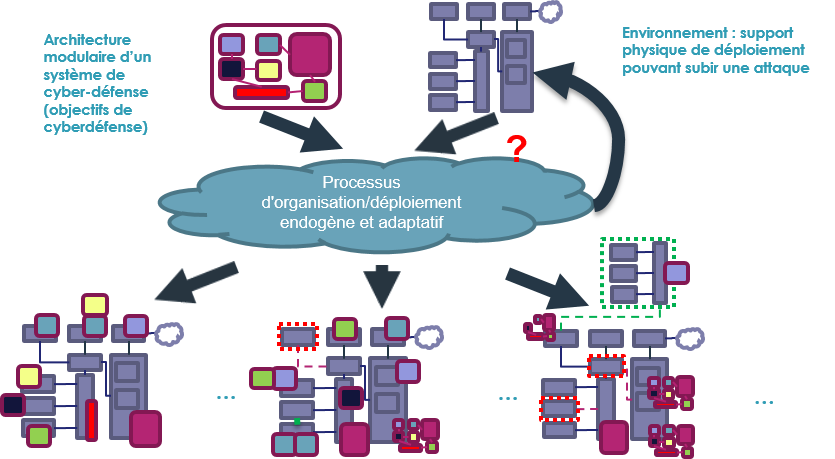
\includegraphics[width=0.9\columnwidth]{images/objectifs.png}
            \includesvg[width=0.8\columnwidth]{images/MARL_cyberdefense.svg}
            \caption{Une vue du modèle Dec-POMDP pour l'apprentissage par renforcement multi-agents (MARL)}
            \label{fig:mon_étiquette}
        \end{figure}

    \end{variableblock}

\end{column}

\separatorcolumn

\hspace{-1ex}

\begin{column}{\colwidth}

\begin{variableblock}{Objectif de recherche pour résoudre}{bg=lightgray,fg=black}{bg=lightgray,fg=black}

    \headingNoLine{Préoccupation} : un processus de conception itératif de SMA est coûteux
    \begin{itemize}
        \item \textbf{Nécessite expérience} : connaissance minimale de l'environnement mais complexe ;
        \item \textbf{Prend beaucoup de temps} : plusieurs conceptions mais contraintes de temps ;
        \item \textbf{Apprentissage limité} accès/expérimentation restreints, peu d'experts\dots
    \end{itemize}

    \headingNoLine{Partial Relation between Agents' History and Organizational Model (PRAHOM)} :
    \begin{itemize}
        \item S'appuie sur MARL pour trouver les politiques optimales des agents ;
        \item Analyse comportements en spécifications organisationnelles (roles, objectifs).
              % \item Fournit automatiquement des spécifications organisationnelles pertinentes et compréhensibles
              % \item Les concepteurs peuvent intégrer des contraintes de conception
    \end{itemize}

    \quad $\Longrightarrow$ \headingNoLine{Approche d'ingénierie de modèle organisationnel assistée (AOMEA)}

    \begin{figure}
        \centering
        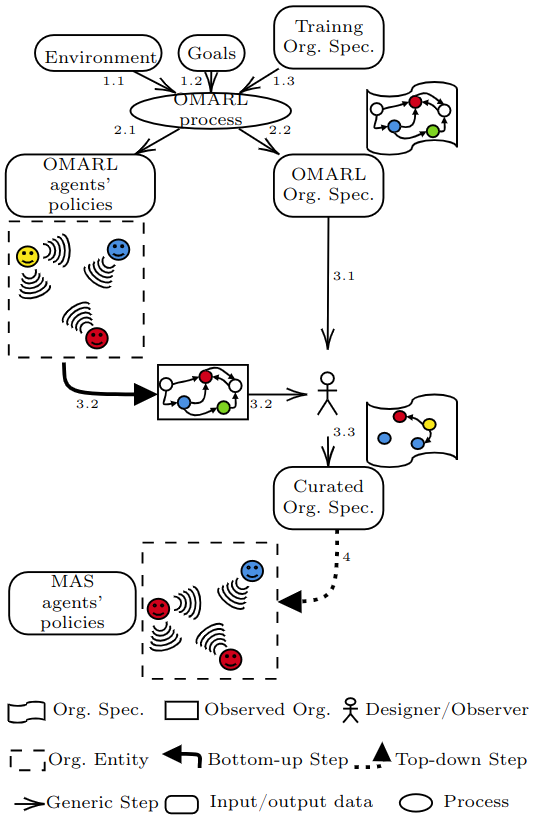
\includegraphics[width=0.55\linewidth]{figures/AOMEA_illustrative_view.png}
        \caption{Vue illustrative de l'AOMEA : Assisted Organizational MAS Engineering Approach}
        \label{fig:mon_étiquette}
    \end{figure}

    % \vspace{-0.8ex}
    \vspace{-2ex}

\end{variableblock}

\begin{variableblock}{Objectif de recherche pour mettre en œuvre}{bg=lightorange,fg=black}{bg=lightorange,fg=black}

\headingNoLine{Implémentation du modèle $\rightarrow$ CybMASDE} :

\begin{itemize}
    \item création/chargement/enregistrement d'un environnement spécifié avec des agents
    \item lancer l'exécution des agents de cet environnement en simulation/émulation
    \item visualisation de l'environnement réseau sous forme de graphique
\end{itemize}

\begin{figure}
    \centering
    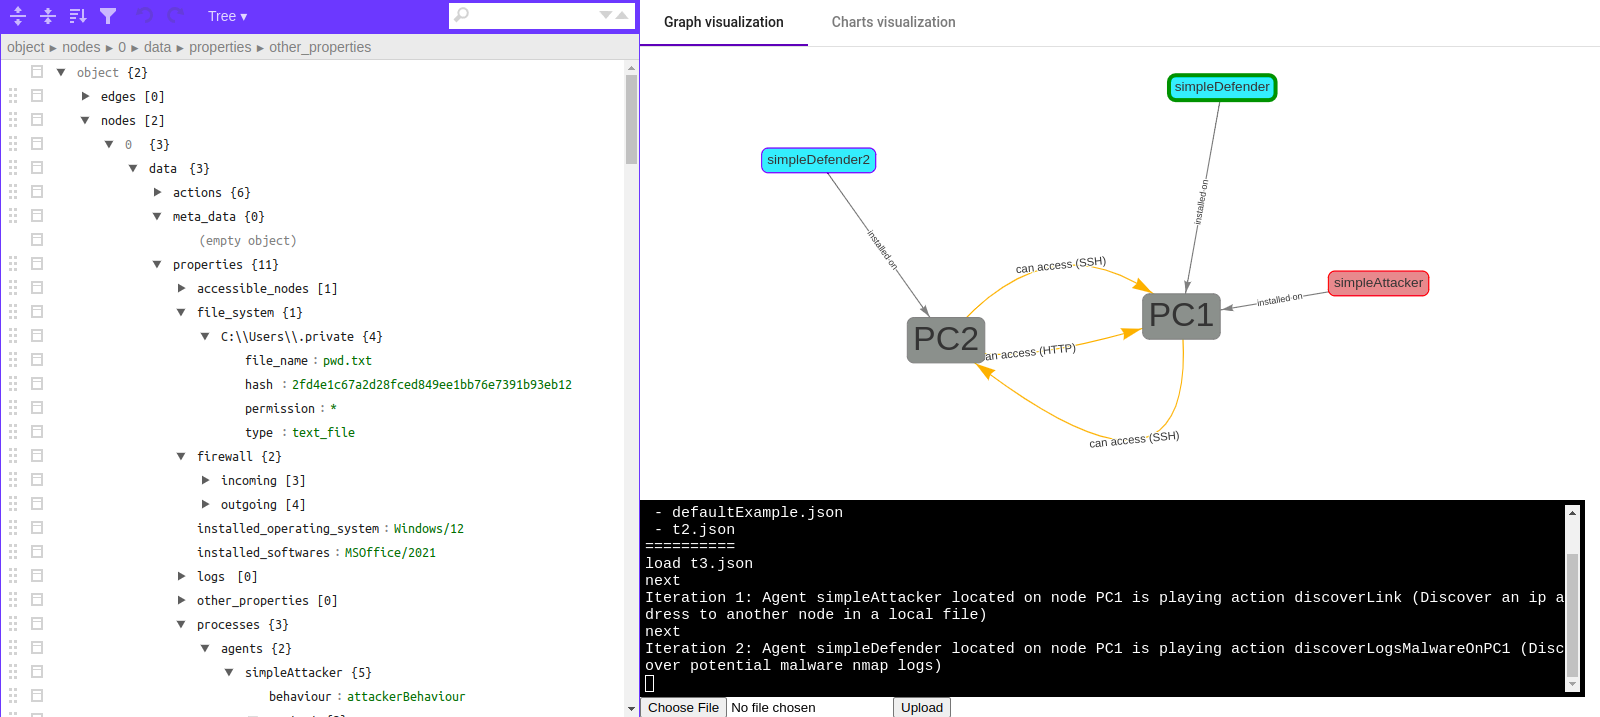
\includegraphics[width=0.8\linewidth]{images/interface_CybMASDE.png}
    \caption{Présentation de Cyberdefense Multi-Agent System Development Environment}
    \label{fig:interface_simulateur}
\end{figure}

\headingNoLine{Implémentation de la résolution en tant que bibliothèque :} nous avons proposé le \textit{PRAHOM PettingZoo Wrapper} :

\begin{tabularx}{\linewidth}{p{32cm}p{7cm}}
{


\tikzset{every picture/.style={line width=0.75pt}} %set default line width to 0.75pt        

\begin{tikzpicture}[x=0.75pt,y=0.75pt,yscale=-1,xscale=1]
%uncomment if require: \path (0,1656); %set diagram left start at 0, and has height of 1656

%Straight Lines [id:da39585146483301226] 
\draw [fill={rgb, 255:red, 155; green, 155; blue, 155 }  ,fill opacity=0.3 ][line width=1.5]    (262,1077.44) -- (262,1088) -- (130,1088) -- (130,1077.44) -- (42,1077.44) -- (42,998.04) -- (42,744) -- (344,744) -- (344,1077.51) -- cycle ;
%Shape: Rectangle [id:dp15141215707199196] 
\draw  [fill={rgb, 255:red, 184; green, 233; blue, 134 }  ,fill opacity=0.54 ] (46,941.55) -- (197.88,941.55) -- (197.88,1070) -- (46,1070) -- cycle ;
%Shape: Rectangle [id:dp6360114669768389] 
\draw  [fill={rgb, 255:red, 80; green, 227; blue, 194 }  ,fill opacity=0.27 ] (204.48,829.34) -- (338,829.34) -- (338,1073.92) -- (204.48,1073.92) -- cycle ;
%Straight Lines [id:da060910289882972535] 
\draw [line width=0.75]    (118.82,1060.45) -- (118.82,1080.99) ;
\draw [shift={(118.82,1083.99)}, rotate = 270] [fill={rgb, 255:red, 0; green, 0; blue, 0 }  ][line width=0.08]  [draw opacity=0] (8.93,-4.29) -- (0,0) -- (8.93,4.29) -- cycle    ;
%Straight Lines [id:da567561296770805] 
\draw [line width=1.5]    (188.58,1051.05) -- (200.95,1051.05) -- (200,868.05) -- (214,868.05) ;
\draw [shift={(218,868.05)}, rotate = 180] [fill={rgb, 255:red, 0; green, 0; blue, 0 }  ][line width=0.08]  [draw opacity=0] (11.61,-5.58) -- (0,0) -- (11.61,5.58) -- cycle    ;
%Straight Lines [id:da27635620179975406] 
\draw [line width=0.75]    (276,1060.45) -- (276,1081) ;
\draw [shift={(276,1084)}, rotate = 270] [fill={rgb, 255:red, 0; green, 0; blue, 0 }  ][line width=0.08]  [draw opacity=0] (8.93,-4.29) -- (0,0) -- (8.93,4.29) -- cycle    ;
%Straight Lines [id:da08883699834879355] 
\draw [line width=0.75]    (276,992) -- (276,1027) ;
\draw [shift={(276,1030)}, rotate = 270] [fill={rgb, 255:red, 0; green, 0; blue, 0 }  ][line width=0.08]  [draw opacity=0] (8.93,-4.29) -- (0,0) -- (8.93,4.29) -- cycle    ;
%Straight Lines [id:da8779234517114483] 
\draw [line width=1.5]    (136,734) -- (135.88,745.84) ;
\draw [shift={(135.84,749.84)}, rotate = 270.59] [fill={rgb, 255:red, 0; green, 0; blue, 0 }  ][line width=0.08]  [draw opacity=0] (11.61,-5.58) -- (0,0) -- (11.61,5.58) -- cycle    ;
%Straight Lines [id:da43837040952509776] 
\draw [line width=1.5]  [dash pattern={on 1.69pt off 2.76pt}]  (244,734) -- (244,745.84) ;
\draw [shift={(244,749.84)}, rotate = 270] [fill={rgb, 255:red, 0; green, 0; blue, 0 }  ][line width=0.08]  [draw opacity=0] (11.61,-5.58) -- (0,0) -- (11.61,5.58) -- cycle    ;
%Shape: Ellipse [id:dp7999411998489565] 
\draw   (43.18,1100.6) .. controls (43.18,1099.21) and (44.23,1098.08) .. (45.53,1098.08) .. controls (46.83,1098.08) and (47.89,1099.21) .. (47.89,1100.6) .. controls (47.89,1101.99) and (46.83,1103.12) .. (45.53,1103.12) .. controls (44.23,1103.12) and (43.18,1101.99) .. (43.18,1100.6) -- cycle ;
%Straight Lines [id:da7827154744519647] 
\draw    (45.53,1103.12) -- (45.53,1109.43) ;
%Straight Lines [id:da757553550080027] 
\draw    (45.53,1109.43) -- (42,1115.73) ;
%Straight Lines [id:da12186027632053076] 
\draw    (45.53,1109.43) -- (49.06,1115.73) ;
%Straight Lines [id:da8177170825815439] 
\draw    (49.06,1105.64) -- (42,1105.64) ;

%Straight Lines [id:da6711978114234527] 
\draw [line width=1.5]    (196.97,1100.04) -- (215.93,1100.04) ;
\draw [shift={(219.93,1100.04)}, rotate = 180] [fill={rgb, 255:red, 0; green, 0; blue, 0 }  ][line width=0.08]  [draw opacity=0] (11.61,-5.58) -- (0,0) -- (11.61,5.58) -- cycle    ;
%Shape: Rectangle [id:dp565997856178448] 
\draw   (269.27,1104.34) -- (294,1104.34) -- (294,1122) -- (269.27,1122) -- cycle ;
%Rounded Rect [id:dp21323776879671108] 
\draw   (112.97,1102.59) .. controls (112.97,1100.64) and (114.55,1099.06) .. (116.5,1099.06) -- (134.16,1099.06) .. controls (136.11,1099.06) and (137.7,1100.64) .. (137.7,1102.59) -- (137.7,1113.18) .. controls (137.7,1115.13) and (136.11,1116.71) .. (134.16,1116.71) -- (116.5,1116.71) .. controls (114.55,1116.71) and (112.97,1115.13) .. (112.97,1113.18) -- cycle ;
%Straight Lines [id:da0858907343631472] 
\draw [line width=0.75]    (68.58,1038.32) -- (68.58,1034.8) -- (68.58,1029) ;
\draw [shift={(68.58,1026)}, rotate = 90] [fill={rgb, 255:red, 0; green, 0; blue, 0 }  ][line width=0.08]  [draw opacity=0] (8.93,-4.29) -- (0,0) -- (8.93,4.29) -- cycle    ;
%Straight Lines [id:da5873937258535422] 
\draw [line width=1.5]  [dash pattern={on 1.69pt off 2.76pt}]  (330,736) -- (329.16,789.15) ;
\draw [shift={(329.09,793.15)}, rotate = 270.91] [fill={rgb, 255:red, 0; green, 0; blue, 0 }  ][line width=0.08]  [draw opacity=0] (11.61,-5.58) -- (0,0) -- (11.61,5.58) -- cycle    ;
%Straight Lines [id:da4772036045501553] 
\draw [line width=1.5]    (50,738) -- (50,807.74) ;
\draw [shift={(50,811.74)}, rotate = 270] [fill={rgb, 255:red, 0; green, 0; blue, 0 }  ][line width=0.08]  [draw opacity=0] (11.61,-5.58) -- (0,0) -- (11.61,5.58) -- cycle    ;
%Straight Lines [id:da9532226437940816] 
\draw [line width=1.5]  [dash pattern={on 1.69pt off 2.76pt}]  (197.56,1113.77) -- (216.51,1113.77) ;
\draw [shift={(220.51,1113.77)}, rotate = 180] [fill={rgb, 255:red, 0; green, 0; blue, 0 }  ][line width=0.08]  [draw opacity=0] (11.61,-5.58) -- (0,0) -- (11.61,5.58) -- cycle    ;
%Shape: Boxed Line [id:dp7740313150184794] 
\draw [line width=0.75]    (152,988) -- (151.97,1037) ;
\draw [shift={(151.96,1040)}, rotate = 270.04] [fill={rgb, 255:red, 0; green, 0; blue, 0 }  ][line width=0.08]  [draw opacity=0] (8.93,-4.29) -- (0,0) -- (8.93,4.29) -- cycle    ;
%Straight Lines [id:da02758195492613358] 
\draw    (152,992) -- (152,1036) ;
%Straight Lines [id:da10022352286826108] 
\draw    (276,880) -- (276,884) ;
%Straight Lines [id:da39235168455073555] 
\draw    (276,914) -- (276,925) ;
\draw [shift={(276,928)}, rotate = 270] [fill={rgb, 255:red, 0; green, 0; blue, 0 }  ][line width=0.08]  [draw opacity=0] (8.93,-4.29) -- (0,0) -- (8.93,4.29) -- cycle    ;


% Text Node
\draw (225,1111) node [anchor=north west][inner sep=0.75pt]   [align=left] {{\scriptsize optionel}};
% Text Node
\draw (223,1095) node [anchor=north west][inner sep=0.75pt]   [align=left] {{\scriptsize Input/Output}};
% Text Node
\draw (297,1094) node [anchor=north west][inner sep=0.75pt]   [align=left] {{\scriptsize Donnés}\\{\scriptsize input/ouput}};
% Text Node
\draw (142,1104) node [anchor=north west][inner sep=0.75pt]   [align=left] {{\scriptsize Processus}};
% Text Node
\draw (53,1103) node [anchor=north west][inner sep=0.75pt]   [align=left] {{\scriptsize Concepteur}};
% Text Node
\draw  [fill={rgb, 255:red, 255; green, 255; blue, 255 }  ,fill opacity=1 ]  (216,988.5) .. controls (216,981.6) and (222.27,976) .. (230,976) -- (321,976) .. controls (328.73,976) and (335,981.6) .. (335,988.5) .. controls (335,995.4) and (328.73,1001) .. (321,1001) -- (230,1001) .. controls (222.27,1001) and (216,995.4) .. (216,988.5) -- cycle  ;
\draw (275.5,988.5) node   [align=left] {\begin{minipage}[lt]{78.33pt}\setlength\topsep{0pt}
\begin{center}
{\footnotesize \textbf{Identifer avec defs.}}
\end{center}

\end{minipage}};
% Text Node
\draw  [fill={rgb, 255:red, 255; green, 255; blue, 255 }  ,fill opacity=1 ]  (213,940.5) .. controls (213,933.6) and (219.27,928) .. (227,928) -- (324,928) .. controls (331.73,928) and (338,933.6) .. (338,940.5) .. controls (338,947.4) and (331.73,953) .. (324,953) -- (227,953) .. controls (219.27,953) and (213,947.4) .. (213,940.5) -- cycle  ;
\draw (275.5,940.5) node   [align=left] {\begin{minipage}[lt]{82.41pt}\setlength\topsep{0pt}
\begin{center}
{\footnotesize \textbf{Identifer avec relat}\textsuperscript{os}}
\end{center}

\end{minipage}};
% Text Node
\draw  [fill={rgb, 255:red, 255; green, 255; blue, 255 }  ,fill opacity=1 ]  (214,1030) -- (331,1030) -- (331,1060) -- (214,1060) -- cycle  ;
\draw (272.5,1045) node   [align=left] {\begin{minipage}[lt]{76.91pt}\setlength\topsep{0pt}
\begin{center}
{\footnotesize Specs. Orgs. Générées}
\end{center}

\end{minipage}};
% Text Node
\draw  [fill={rgb, 255:red, 255; green, 255; blue, 255 }  ,fill opacity=1 ]  (243,884) -- (306,884) -- (306,914) -- (243,914) -- cycle  ;
\draw (274.5,899) node   [align=left] {\begin{minipage}[lt]{40.23pt}\setlength\topsep{0pt}
\begin{center}
{\small $\displaystyle \{H_{joint}\} \ $}
\end{center}

\end{minipage}};
% Text Node
\draw  [fill={rgb, 255:red, 255; green, 255; blue, 255 }  ,fill opacity=1 ]  (218,866.87) .. controls (218,859.69) and (224.27,853.87) .. (232,853.87) -- (319,853.87) .. controls (326.73,853.87) and (333,859.69) .. (333,866.87) .. controls (333,874.05) and (326.73,879.87) .. (319,879.87) -- (232,879.87) .. controls (224.27,879.87) and (218,874.05) .. (218,866.87) -- cycle  ;
\draw (275.5,866.87) node   [align=left] {\begin{minipage}[lt]{75.66pt}\setlength\topsep{0pt}
\begin{center}
{\footnotesize \textbf{Générer historiques}}
\end{center}

\end{minipage}};
% Text Node
\draw (132.64,1072) node [anchor=north west][inner sep=0.75pt]   [align=left] {PRAHOM Wrapper};
% Text Node
\draw (272,839.45) node   [align=left] {\begin{minipage}[lt]{87.07pt}\setlength\topsep{0pt}
\begin{center}
{\footnotesize \textbf{Générat° Specs. Org.}}
\end{center}

\end{minipage}};
% Text Node
\draw  [fill={rgb, 255:red, 255; green, 255; blue, 255 }  ,fill opacity=1 ]  (48.47,1010) .. controls (48.47,1002.27) and (54.74,996) .. (62.47,996) -- (180.47,996) .. controls (188.2,996) and (194.47,1002.27) .. (194.47,1010) -- (194.47,1012) .. controls (194.47,1019.73) and (188.2,1026) .. (180.47,1026) -- (62.47,1026) .. controls (54.74,1026) and (48.47,1019.73) .. (48.47,1012) -- cycle  ;
\draw (121.47,1011) node   [align=left] {\begin{minipage}[lt]{96.56pt}\setlength\topsep{0pt}
\begin{center}
{\footnotesize PPO - \textit{StableBaseLines3}}
\end{center}

\end{minipage}};
% Text Node
\draw (119.29,947.71) node   [align=left] {\begin{minipage}[lt]{94.87pt}\setlength\topsep{0pt}
\begin{center}
{\footnotesize \textbf{Entrainement}}
\end{center}

\end{minipage}};
% Text Node
\draw  [fill={rgb, 255:red, 255; green, 255; blue, 255 }  ,fill opacity=1 ]  (48.47,960.84) -- (189.47,960.84) -- (189.47,991.84) -- (48.47,991.84) -- cycle  ;
\draw (118.97,976.34) node   [align=left] {\begin{minipage}[lt]{93.07pt}\setlength\topsep{0pt}
\begin{center}
\textbf{{\footnotesize Contraintes sur politiques}}
\end{center}

\end{minipage}};
% Text Node
\draw  [fill={rgb, 255:red, 255; green, 255; blue, 255 }  ,fill opacity=1 ]  (48.47,1038.27) -- (189.47,1038.27) -- (189.47,1068.27) -- (48.47,1068.27) -- cycle  ;
\draw (118.97,1053.27) node   [align=left] {\begin{minipage}[lt]{93.07pt}\setlength\topsep{0pt}
\begin{center}
{\small $\displaystyle \Pi _{joint,\ entrainement} \ $}
\end{center}

\end{minipage}};
% Text Node
\draw  [fill={rgb, 255:red, 248; green, 231; blue, 28 }  ,fill opacity=0.37 ]  (46,812.19) -- (194,812.19) -- (194,938.19) -- (46,938.19) -- cycle  ;
\draw (120,875.19) node   [align=left] {\begin{minipage}[lt]{97.92pt}\setlength\topsep{0pt}
\begin{center}
\textbf{{\footnotesize Configuration}}
\end{center}
{\footnotesize \underline{\textit{Entrainement contraint }:}}\\{\footnotesize intégrat° contraintes, nb itérat°, CPU, temps, récompense seuil...}\\{\footnotesize \underline{\textit{Determinat° Specs. Org.} :}}\\{\footnotesize specs. org. output, techniques utilisées, générer figures...}
\end{minipage}};
% Text Node
\draw  [fill={rgb, 255:red, 248; green, 231; blue, 28 }  ,fill opacity=0.37 ]  (206,746) -- (321,746) -- (321,792) -- (206,792) -- cycle  ;
\draw (263.5,769) node   [align=left] {\begin{minipage}[lt]{75.55pt}\setlength\topsep{0pt}
\begin{center}
\textbf{{\footnotesize Relations entre \textit{historiques }et\textit{ specs. orgs.}}}
\end{center}

\end{minipage}};
% Text Node
\draw  [fill={rgb, 255:red, 248; green, 231; blue, 28 }  ,fill opacity=0.37 ]  (206,794) -- (338,794) -- (338,826) -- (206,826) -- cycle  ;
\draw (272,810) node   [align=left] {\begin{minipage}[lt]{87.04pt}\setlength\topsep{0pt}
\begin{center}
{\footnotesize \textbf{Contraintes specs. org.} avec agents }
\end{center}

\end{minipage}};
% Text Node
\draw  [fill={rgb, 255:red, 248; green, 231; blue, 28 }  ,fill opacity=0.37 ]  (57,746) -- (202,746) -- (202,806) -- (57,806) -- cycle  ;
\draw (129.5,776) node   [align=left] {\begin{minipage}[lt]{96.07pt}\setlength\topsep{0pt}
\begin{center}
{\footnotesize \textbf{Env. PettingZoo}}
\end{center}
{\footnotesize agents ; transitions ; actions ; observations ; récompense ; horizon...}
\end{minipage}};
% Connection
\draw    (275.5,953) -- (275.5,973) ;
\draw [shift={(275.5,976)}, rotate = 270] [fill={rgb, 255:red, 0; green, 0; blue, 0 }  ][line width=0.08]  [draw opacity=0] (8.93,-4.29) -- (0,0) -- (8.93,4.29) -- cycle    ;

\end{tikzpicture}} &
{
        \vspace{1.8ex}
        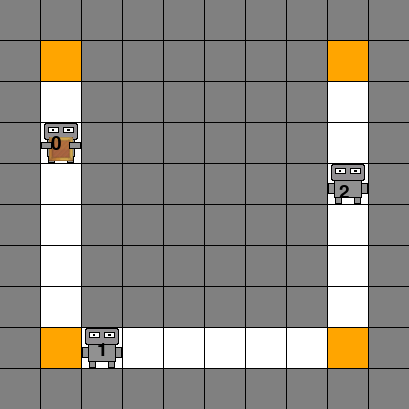
\includegraphics[width=1.0\linewidth]{figures/moving_company_v0.png}} \\
\end{tabularx}

\vspace{-2ex}

\end{variableblock}

\begin{variableblock}{Perspectives}{bg=lightgray,fg=black}{bg=lightgray,fg=black}
    \vspace{-1ex}
    \begin{itemize}
        \item \textbf{Meilleure explicabilité} : Grands modèles de langage (LLM)
        \item \textbf{Réduire l'écart entre la simulation et la réalité} : amélioration de l'émulation \& identification du système
        \item \textbf{Évaluation \& Généricité} : Études de cas industrielles \& académiques
    \end{itemize}
\end{variableblock}

\end{column}
\separatorcolumn


\end{columns}
\end{frame}

\end{document}